%!TeX root=../tese.tex

%% ------------------------------------------------------------------------- %%
\chapter{Metodologia}
\label{cap:metodologia}

Neste capítulo será detalhado o método que se deseja utilizar para realizar a
detecção de anomalias que esta pesquisa propõe.

Para a análise do comportamento da aplicação serão coletados dados de aplicações
web de forma não invasiva. O principal motivo para utilizar estes dados está na
facilidade com que eles podem ser obtidos sem a necessidade que as aplicações
tenham que ser instrumentadas para dar informações de seu comportamento.

Para obtenção destes dados serão utilizados registros das requisições e respostas
intermediadas por balanceadores de carga, os quais contém o mínimo de informação
necessária para a avaliação proposta, e tratando assim a aplicação como uma caixa
preta (figura 3.1) da qual não precisamos conhecer nenhum detalhe interno.

\begin{figure}
  \centering
  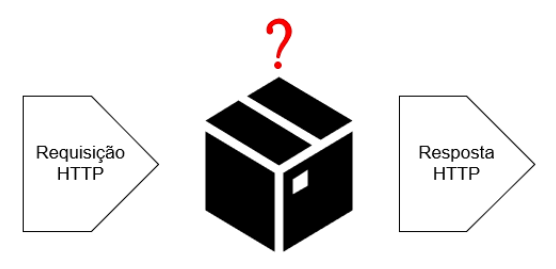
\includegraphics[width=.7\textwidth]{figura4}
  \caption{Aplicação tratada como uma caixa preta.\label{fig:aplicacao-tratada-como-uma-caixa-preta}}
\end{figure}

Outro motivo para esta abordagem é a possibilidade deste mecanismo ser genérico o
suficiente para se tornar um serviço de monitoramento de outros serviços, o que é
bastante interessante para a empresa HP Inc., da qual sou funcionário, que irá
fornecer dados de aplicações em produção para realização de testes.


Na figura 3.2 é descrita a arquitetura de uma aplicação real que realiza o
armazenamento de arquivos em diversos provedores.

\begin{figure}
  \centering
  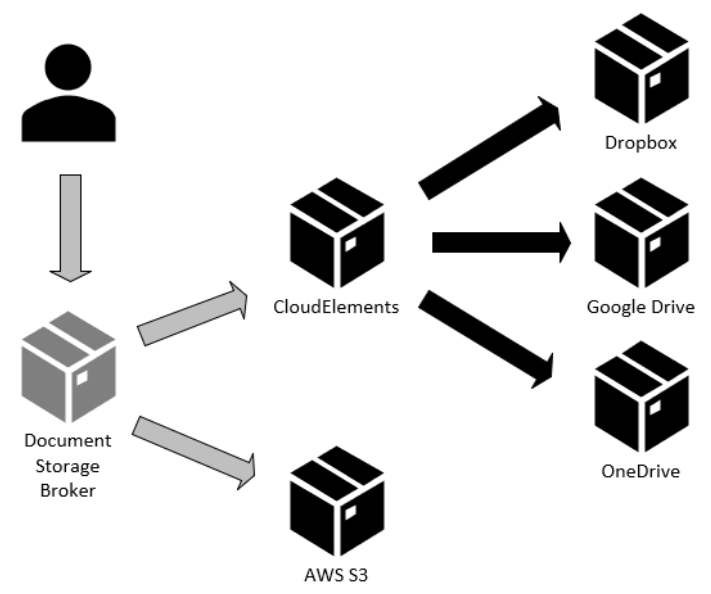
\includegraphics[width=.7\textwidth]{figura5}
  \caption{Interação entre serviços do \textit{Document Storage Broker}.\label{fig:document-storage-broker}}
\end{figure}

O serviço Document Storage Broker recebe requisições dos usuários e encaminha para
o serviço de outra empresa chamada CloudElements\footnote[7]{\url{http://www.cloud-elements.com}},
intermediária de outros serviços como Dropbox, Google Drive ou OneDrive, ou para o
serviço de armazenamento de arquivos da AWS, conforme parâmetros enviados pelo
usuário.

Nesta arquitetura seria possível utilizar a metodologia apresentada tanto nas
requisições recebidas pelo Document Storage Broker quanto nas que são enviadas
para as empresas CloudElements e AWS.

De posse destes dados serão utilizadas técnicas de aprendizado de máquina de
detecção de anomalias e regressão logística para tentar responder às seguintes
questões:

\begin{enumerate}
  \item A aplicação web está se comportando de forma anômala?
  \item Qual a causa provável da anomalia?
\end{enumerate}

Alguns cenários esperados para anomalia e causa são: aumento de tempo de resposta
dado um aumento no número de usuários acessando a aplicação, e aumento na
quantidade de erros dada uma falha em uma dependência da aplicação.

Os dados a serem avaliados inicialmente serão provenientes de uma aplicação de
teste com cenário de sobrecarga e posteriormente serão realizados testes utilizando
dados anonimizados de uma aplicação em produção da empresa HP Inc., os quais estão
pendentes de autorização da empresa para sua publicação.

Caso não seja permitida a publicação dos registros da HP Inc., serão publicados
registros novos da aplicação de teste que irão simular os cenários que desejamos
detectar.
